\subsection{RAID 50}

RAID 5+0 (RAID 50) es un RAID compuesto que combina RAID 5 y RAID 0.

Conceptualmente, primero se crean dos o más arreglos RAID 5, cada uno con su propia paridad distribuida. Luego, esos arreglos se combinan mediante RAID 0, distribuyendo los datos entre ellos para incrementar el rendimiento.

Por ejemplo, un arreglo RAID 50 con seis discos tendría una configuración como la representada en la figura \ref{fig:raid50}.

\begin{figure}[!ht]
  \centering
  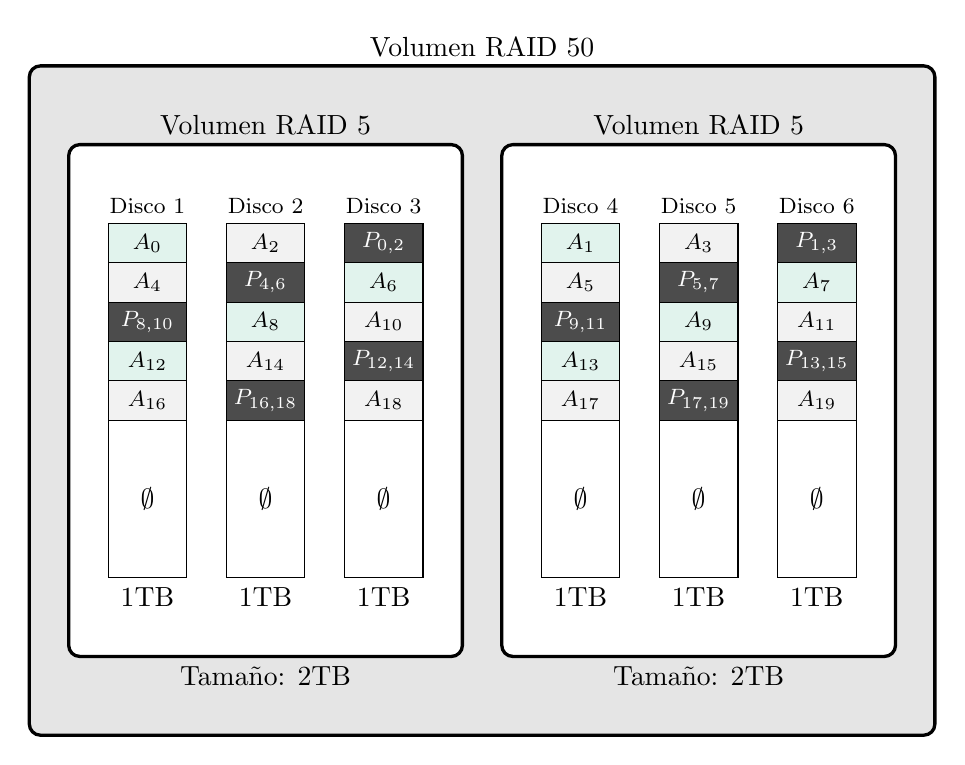
\begin{tikzpicture}
    % RAID 0
    \draw[very thick, rounded corners, fill=gray!20] (-1,-4) rectangle (10.5,4.5);
    \node[above] at (4.75,4.5) {Volumen RAID 50};

    % RAID 5
    \draw[very thick,rounded corners,fill=white] (-0.5,-3) rectangle (4.5,3.5);
    \node[above] at (2,3.5) {Volumen RAID 5};
    \node[below] at (2,-3) {Tamaño: 2TB};

    \draw[very thick,rounded corners,fill=white] (5,-3) rectangle (10,3.5);
    \node[above] at (7.5,3.5) {Volumen RAID 5};
    \node[below] at (7.5,-3) {Tamaño: 2TB};

    \node[above,font=\footnotesize] at (0.5,2.5) {Disco 1};
    \foreach \y\t\c in {
        0/A_{16}/gray!10,
        0.5/A_{12}/white!95!blue!93!green,
        1/\color{white}P_{8,10}/black!70,
        1.5/A_4/gray!10,
        2/A_0/white!95!blue!93!green}{
      \draw[fill=\c] (0,\y) rectangle node[font=\footnotesize]{\(\t\)} (1,{0.5+\y});
    }
    \draw (0,0) rectangle node{\(\emptyset\)} (1,-2);
    \node[below] at (0.5,-2) {1TB};

    \node[above,font=\footnotesize] at (2,2.5) {Disco 2};
    \foreach \y\t\c in {
        0/\color{white}P_{16,18}/black!70,
        0.5/A_{14}/gray!10,
        1/A_8/white!95!blue!93!green,
        1.5/\color{white}P_{4,6}/black!70,
        2/A_2/gray!10}{
      \draw[fill=\c] (1.5,\y) rectangle node[font=\footnotesize]{\(\t\)} (2.5,{0.5+\y});
    }
    \draw (1.5,0) rectangle node{\(\emptyset\)} (2.5,-2);
    \node[below] at (2,-2) {1TB};

    \node[above,font=\footnotesize] at (3.5,2.5) {Disco 3};
    \foreach \y\t\c in {
        0/A_{18}/gray!10,
        0.5/\color{white}P_{12,14}/black!70,
        1/A_{10}/gray!10,
        1.5/A_6/white!95!blue!93!green,
        2/\color{white}P_{0,2}/black!70}{
      \draw[fill=\c] (3,\y) rectangle node[font=\footnotesize]{\(\t\)} (4,{0.5+\y});
    }
    \draw (3,0) rectangle node{\(\emptyset\)} (4,-2);
    \node[below] at (3.5,-2) {1TB};


    \node[above,font=\footnotesize] at (6,2.5) {Disco 4};
    \foreach \y\t\c in {
        0/A_{17}/gray!10,
        0.5/A_{13}/white!95!blue!93!green,
        1/\color{white}P_{9,11}/black!70,
        1.5/A_5/gray!10,
        2/A_1/white!95!blue!93!green}{
      \draw[fill=\c] (5.5,\y) rectangle node[font=\footnotesize]{\(\t\)} (6.5,{0.5+\y});
    }
    \draw (5.5,0) rectangle node{\(\emptyset\)} (6.5,-2);
    \node[below] at (6,-2) {1TB};

    \node[above,font=\footnotesize] at (7.5,2.5) {Disco 5};
    \foreach \y\t\c in {
        0/\color{white}P_{17,19}/black!70,
        0.5/A_{15}/gray!10,
        1/A_9/white!95!blue!93!green,
        1.5/\color{white}P_{5,7}/black!70,
        2/A_3/gray!10}{
      \draw[fill=\c] (7,\y) rectangle node[font=\footnotesize]{\(\t\)} (8,{0.5+\y});
    }
    \draw (7,0) rectangle node{\(\emptyset\)} (8,-2);
    \node[below] at (7.5,-2) {1TB};

    \node[above,font=\footnotesize] at (9,2.5) {Disco 6};
    \foreach \y\t\c in {
        0/A_{19}/gray!10,
        0.5/\color{white}P_{13,15}/black!70,
        1/A_{11}/gray!10,
        1.5/A_7/white!95!blue!93!green,
        2/\color{white}P_{1,3}/black!70}{
        \draw[fill=\c] (8.5,\y) rectangle node[font=\footnotesize]{\(\t\)} (9.5,{0.5+\y});
    }
    \draw (8.5,0) rectangle node{\(\emptyset\)} (9.5,-2);
    \node[below] at (9,-2) {1TB};

  \end{tikzpicture}
  \caption{Tamaño del volumen de RAID 50: 4TB.}
  \label{fig:raid50}
\end{figure}

Cada RAID 5 funciona de manera independiente, manteniendo su propia información de paridad. Para el RAID 0 superior, cada uno de esos arreglos se comporta como si fuera un único disco lógico.

\paragraph{Características}
\begin{itemize}
  \item Combina el alto rendimiento del striping (RAID 0) con la redundancia mediante paridad de RAID 5.
  \item Requiere al menos seis discos (dos grupos RAID 5 de tres discos cada uno).
  \item La capacidad útil es la suma de las capacidades útiles de cada RAID 5.
\end{itemize}

\paragraph{Tolerancia a fallos}
Cada subarreglo RAID 5 puede soportar la falla de un disco.

Por ello, un RAID 50 puede tolerar la falla de más de un disco, siempre que las fallas ocurran en grupos RAID 5 distintos.

Por ejemplo, si existen dos grupos RAID 5:
\begin{itemize}
  \item Puede fallar un disco del primer grupo y otro del segundo grupo.
  \item Si fallan dos discos del mismo grupo RAID 5, ese grupo deja de funcionar y, como el RAID 0 depende de todos los grupos, se pierde el volumen completo.
\end{itemize}
En general, la tolerancia máxima depende de cómo se distribuyan las fallas entre los distintos subarreglos.

RAID 50 ofrece un mejor equilibrio entre rendimiento y disponibilidad que un único RAID 5 de gran tamaño:
\begin{itemize}
  \item El RAID 0 incrementa el rendimiento al distribuir las operaciones entre varios grupos.
  \item Cada RAID 5 mantiene su propia paridad, por lo que las reconstrucciones afectan únicamente al grupo donde ocurrió la falla y no a todo el arreglo.
\end{itemize}

\begin{table}[!ht]
  \centering
  \begin{tabular}{l|c}
    Cantidad de discos mínima & 6 \\\hline
    Cantidad de discos que pueden fallar & 2 (1\(\times\)RAID 5) \\ \hline
    Velocidad de escritura relativa a un disco & \(M\times\frac{\text{VDisco}}{\text{Cant. Oper.}}\)~[MB/s] \\\hline
    Velocidad de escritura ponderada & 3 \\ \hline
    Velocidad de lectura relativa a un disco & \(M\times\)VDisco~[MB/s] \\ \hline
    Velocidad de lectura ponderada & 8 \\ \hline
    Costo & Alto
  \end{tabular}
  \caption{Características del RAID 50.}
  \label{tab:raid50}
\end{table}

En el cuadro \ref{tab:raid50} \(M\) es la cantidad de arreglos RAID 5 que tiene el volumen RAID 50. Por ejemplo, en la figura \ref{fig:raid50}, \(M=2\) porque hay dos arreglos RAID 5.
